\chapter{Report and analysis}\label{chap:report}
\section{Project structure}

During model development, it became evident that a systematic approach, outlined by multiple steps within our methodology, is imperative to achieve optimal outcomes. Consequently, we opted to configure our project according to the framework illustrated in the graph below, thereby facilitating the division of work into more manageable components.\\

\tikzset{every picture/.style={line width=0.75pt}} 
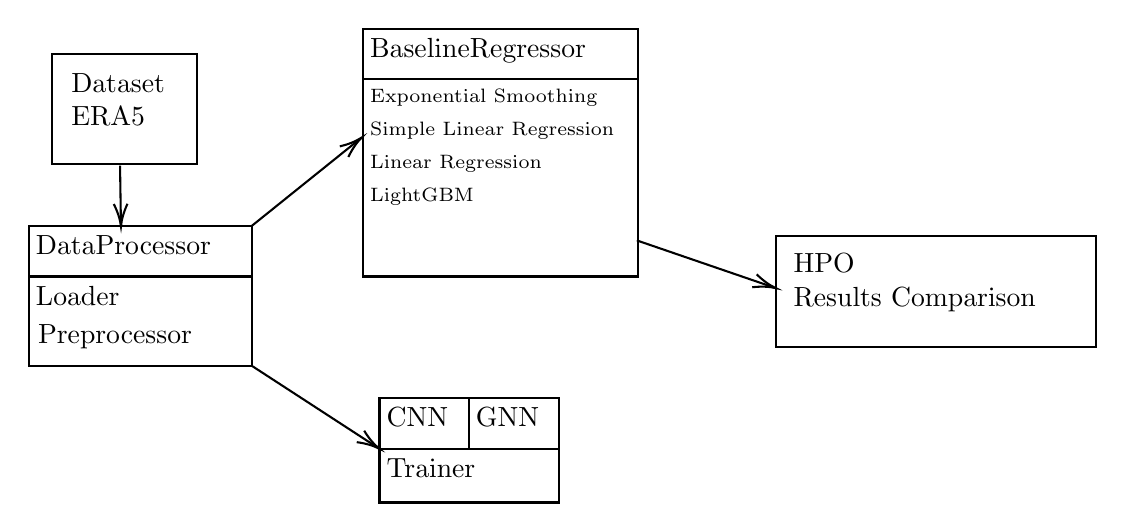
\begin{tikzpicture}[x=0.75pt,y=0.75pt,yscale=-1,xscale=1]
\draw   (49,24) -- (119,24) -- (119,77.4) -- (49,77.4) -- cycle ;
\draw   (38,107) -- (145.47,107) -- (145.47,131.4) -- (38,131.4) -- cycle ;
\draw   (199,12) -- (331.47,12) -- (331.47,36.4) -- (199,36.4) -- cycle ;
\draw   (38,131.4) -- (145.47,131.4) -- (145.47,174.4) -- (38,174.4) -- cycle ;
\draw   (199,36.4) -- (331.47,36.4) -- (331.47,131.4) -- (199,131.4) -- cycle ;
\draw    (82,78) -- (82.42,105.35) ;
\draw [shift={(82.45,107.35)}, rotate = 269.12] [color={rgb, 255:red, 0; green, 0; blue, 0 }  ][line width=0.75]    (10.93,-3.29) .. controls (6.95,-1.4) and (3.31,-0.3) .. (0,0) .. controls (3.31,0.3) and (6.95,1.4) .. (10.93,3.29)   ;
\draw    (145.47,107) -- (196.91,65.65) ;
\draw [shift={(198.47,64.4)}, rotate = 141.21] [color={rgb, 255:red, 0; green, 0; blue, 0 }  ][line width=0.75]    (10.93,-3.29) .. controls (6.95,-1.4) and (3.31,-0.3) .. (0,0) .. controls (3.31,0.3) and (6.95,1.4) .. (10.93,3.29)   ;
\draw   (207,190) -- (293.47,190) -- (293.47,214.4) -- (207,214.4) -- cycle ;
\draw   (207,214.4) -- (293.47,214.4) -- (293.47,240.27) -- (207,240.27) -- cycle ;
\draw    (250.1,190.17) -- (250.1,214.17) ;
\draw    (145.47,174.4) -- (205.32,213.31) ;
\draw [shift={(207,214.4)}, rotate = 213.03] [color={rgb, 255:red, 0; green, 0; blue, 0 }  ][line width=0.75]    (10.93,-3.29) .. controls (6.95,-1.4) and (3.31,-0.3) .. (0,0) .. controls (3.31,0.3) and (6.95,1.4) .. (10.93,3.29)   ;
\draw   (398,112) -- (552,112) -- (552,165.4) -- (398,165.4) -- cycle ;
\draw    (331,114) -- (396.11,136.35) ;
\draw [shift={(398,137)}, rotate = 198.95] [color={rgb, 255:red, 0; green, 0; blue, 0 }  ][line width=0.75]    (10.93,-3.29) .. controls (6.95,-1.4) and (3.31,-0.3) .. (0,0) .. controls (3.31,0.3) and (6.95,1.4) .. (10.93,3.29)   ;
\draw (57,32) node [anchor=north west][inner sep=0.75pt]   [align=left] {Dataset\\ERA5};
\draw (40,110) node [anchor=north west][inner sep=0.75pt]   [align=left] {DataProcessor};
\draw (40,134.4) node [anchor=north west][inner sep=0.75pt]   [align=left] {Loader};
\draw (41,153) node [anchor=north west][inner sep=0.75pt]   [align=left] {Preprocessor};
\draw (201,15) node [anchor=north west][inner sep=0.75pt]   [align=left] {BaselineRegressor};
\draw (201,39.4) node [anchor=north west][inner sep=0.75pt]   [align=left] {{\scriptsize Exponential Smoothing}\\{\scriptsize Simple Linear Regression}\\{\scriptsize Linear Regression}\\{\scriptsize LightGBM}};
\draw (209,193) node [anchor=north west][inner sep=0.75pt]   [align=left] {CNN \ \ GNN};
\draw (209,217.4) node [anchor=north west][inner sep=0.75pt]   [align=left] {Trainer};
\draw (405,119) node [anchor=north west][inner sep=0.75pt]   [align=left] {HPO \\Results Comparison};
\end{tikzpicture}

\paragraph{Data Processor}  \mbox{} \\
\noindent The Data Processor is responsible for processing and loading input data from the ERA 5 dataset. Its primary components include the Loader and Preprocessor. The Loader's functions encompass loading data and converting units to the appropriate type. The Preprocessor manages the preprocessing of data essential for model training. It's functionality is used widely between baselines and neural nets. You can find additional details regarding preprocessing methods in Chapter \ref{chap:preprocesing}.

\paragraph{Baseline Regressor}\mbox{} \\ 
\noindent The Baseline Regressor is the foundational model that has simple functions for fitting, evaluating, and predicting. Exponential Smoothing, Simple Linear Regression, Linear Regression, and Gradient Boosting all inherit the Baseline Regressor functions and use altered versions of them for their purposes. Details regarding baselines are provided in Chapter \ref{chap:baselines}.

\paragraph{Trainer} \mbox{} \\
\noindent Both of our neural network models have the Trainer component, where all functionality related to training, predicting, and evaluating was implemented.

\paragraph{HPO and Analysis} \mbox{} \\
\noindent Within the Hyperparameter Optimization (HPO) component, we created a pipeline to obtain the best hyperparameters for the baselines, using the Optuna library in Python. Further details are provided in Chapter \ref{chap:hpo}.
Inside the Analysis component all models undergo evaluation for input size length and number of predicted steps. Moreover, the GNN undergoes evaluation for the number of graph layers. The results of this evaluation are presented in Section \ref{chap:analysis}

\paragraph{Experiments} \mbox{} \\
\noindent The Experiments section of our project is dedicated to testing novel methods and ideas aimed at enhancing our models. We check the correlation between the models and assess the possibility of combining the predictions of the topline with our model to improve its performance.

\section{Dataset description}\label{chap:dataset}
% Description of dataset, train, val, test split, resoution of data, generally all details.
As mentioned previously, the data we used came from the Copernicus Climate Change Service (C3S) Climate Data Store (CDS) "ERA5 hourly data on single levels from 1940 to present" dataset \cite{ERA5}. It contains hundreds of different variables, many of which at different pressure levels (different heights above ground, depending on air pressure). Data is available on an hourly basis, from 1940 until today. It is also worth noting that the dataset is updated with a latency of about 5-6 days.

We used a subset of the archive, usually using 3-year period to construct the training, validation and testing datasets each containing a full year. When creating and testing the methods, we used 2019-2021 year span. We mostly did not use 2023, since the entire year has not passed yet for most of our work. In the app and our API, we use data from a week before the date of use, since it was the easiest way to present our work without paying a steep price for appropriately formatted live data.

\begin{table}[!ht]
\centering
\begin{tabular}{|c|c|c|}
     \hline
     Symbol & Quantity & Unit \\
     \hline
     t2m & Temperature at 2m above ground & $^{\circ}$C \\
     sp & Surface pressure & hPa \\
     tcc & Total cloud cover & (0 - 1) \\
     u10 & 10m U wind component & $m/s$ \\
     v10 & 10m V wind component & $m/s$ \\
     tp & Total precipitation & mm \\
     \hline
     lsm & Land-sea mask (not predicted) & (0 - 1) \\
     z & Geopotential (not predicted) & $m^2/s^2$ \\
     \hline
\end{tabular}
\caption{Weather features we considered. Some of the units differ from those provided in the dataset. These have been converted for our convenience}
\label{tab:data_features2}
\end{table}

As mentioned in Table \ref{tab:data_features2}, we used 6 features for prediction and evaluation, and 2 additional variables as bonus data inputs to improve our neural networks. Since the data is divided into 6 hour intervals, this means that we get measurements from 00:00, 06:00, 12:00 and 18:00 of every day -- therefore for all variables except total precipitation, the data has to be downsampled by subsampling. For total precipitation, it is the amount accumulated during the 6 hour window from the previous timestamp.

Since we are focusing just on Poland, we have determined that the coordinates 55$^{\circ}$N 14$^{\circ}$E and 49$^{\circ}$N 25$^{\circ}$E are able to encapsulate the entirety of the country, without leaving much around it -- Poland is quite square (with the exception of the southern border that has a slight slant to it). This is the area that we evaluate our models on.

However, for our neural networks we needed a slightly bigger area to minimize border effects. Additionally, we required the area to create an array with a shape divisible by $2^5$ in order for the U-net architecture to work correctly. This meant that for those we used the coordinates of 55.75$^{\circ}$N 13.25$^{\circ}$E and 48$^{\circ}$N 25$^{\circ}$E to create the dataset (meaning 32x48 grid boxes).

The map is divided into grid boxes of resolution 0.25 by 0.25 degrees. This translates to a square with a side of about 28km at the equator. Due to the shape of the Earth, this means that the boxes are more complex shapes, with the north-south length still being about 28km, and the east-west length being slightly shorter on the northern side than on the southern side, both about 17km in length at our latitude.

The dataset can be easily downloaded from an API \footnote{\url{https://cds.climate.copernicus.eu/cdsapp\#!/dataset/reanalysis-era5-single-levels?tab=form}}, with specified parameters (such as the timeframe, which variables, the area etc.) and returns a special GRIB \footnote{Gridded Binary or General Regularly-distributed Information in Binary form} file. This can then be depackaged into an xarray \cite{hoyer2017xarray} Dataset object by the cfgrib Python library \cite{80908cfgrib}. The needed data can then be extracted as numerical values into a numpy \cite{harris2020array} Array. This way we can easily download and manipulate data as needed.


\section{Data analysis}
In this section, an examination of a set of target features is conducted. It is important to note that the analyzed data represents our test set, i.e. all weather states in Poland throughout 2021, with data collected at 6-hour intervals. Figure \ref{fig:dist} below represents distributions of the occurrence of the features during this period. Detailed statistics related to each feature are presented in Table \ref{tab:stats}.

\begin{figure}[!ht]
    \centering
    \includegraphics[scale=0.4]{figures/feature_dist.pdf}
    \caption{Feature distributions -- year 2021}
    \label{fig:dist}
\end{figure} 

\begin{figure}[!ht]
    \centering
    \begin{tabular}{C{2.5cm}C{2.5cm}C{2.5cm}C{2.5cm}C{2.5cm}}
        \toprule
        & Mean & Standard Deviation & Skewness & Kurtosis \\
        \midrule
        t2m & 8.575639 & 9.021646 & 0.009954 & -0.416774 \\
        sp & 991.730286 & 20.814014 & -1.214771 & 1.940067 \\
        tcc & 0.674897 & 0.359240 & -0.710991 & -1.029664 \\
        u10 & 1.067543 & 2.924007 & 0.145360 & 0.863331 \\
        v10 & 0.368444 & 2.674111 & -0.003036 & 0.357381 \\
        tp & 0.087919 & 0.311576 & 9.773823 & 171.063156 \\
        \bottomrule
    \end{tabular}
    \caption{Feature statistics -- year 2021}
    \label{tab:stats}
\end{figure}

The plots assigned to temperature, and winds seem to be balanced, while the distribution of pressure is a little left skewed. Cloud cover, however, presents a more challenging scenario, it has two distinct peaks close to the extreme values (i.e. no clouds and full cloud cover) -- indicating highly imbalanced distribution. The precipitation feature emerges the most extreme, which is an expected result due to the early indications, e.g. contained in Chapter \ref{sec:fourcastnet}, stating that this is the feature with the most difficult distribution, often not correlated with the others and requiring special treatment.In summary, based on these distributions, target features can be categorized into two groups: those with relatively straightforward distributions (t2m, sp, u10, v10) for which prediction may be less challenging, and those with more intricate distributions, whose prediction might be an extremely difficult task. 


\section{Topline}
We wanted to compare our models to predictions made by a well-established NWP model. We called this the topline (in oppposition to the baselines), since we expect to not beat the results this method provides, but want to get as close as we can to it.
In our search for a reliable and easy to work with topline dataset, we have chosen ECMWF's TIGGE \cite{tigge}. It consists of ensemble forecast data from 13 NWP centers around the world. It was established as part of a global program, THORPEX \cite{bougeault2010thorpex}, that aims to accelerate the improvements of 1-day to 2-week weather forecast accuracy. The data can be easily downloaded from an API \footnote{\url{https://apps.ecmwf.int/datasets/data/tigge/levtype=sfc/type=cf/}}, in the GRIB format. Due to this similarity to the ERA5 dataset, it was very easy to adapt our methods to quickly get quality forecast data that we could compare our models to.

Unfortunately, the forecasts are done every 12 hours, unlike every 6 hours in the case of our models. This meant that we do not have 1-to-1 comparisons as frequently as we would have hoped, but we determined this was still a sufficient way to compare our solutions to a topline model. All of the features we wanted were available, and the area of the dataset can be chosen and is also the same as in the case of ERA5 data we used.

\section{Preprocessing methods}\label{chap:preprocesing}
The data was stored as numpy \cite{harris2020array} Arrays, which made it considerably easier to preprocess. First, we changed the units of temperature to degrees Celsius instead of Kelvin by simply subtracting 273.15. Then, we divided the pressure by 100 to get from Pascals to hectoPascals. Finally, we multiply total precipitation by 1000 to get milimeters from meters. This was done to get more relatable results, as these are the units commonly used when describing weather.

Next, we create overlapping sequences using the sliding window approach of length equal to the sum of model input length and forecasting horizon: $s + h$. The array of sequences has the shape of 
\[
    (sequences, s+h, latitudes, longitudes, features)
\] 
It is then evenly divided into the training, validation, and test sets, which are consequently shuffled.

\subsection{Data Standardisation}
We have the option to standardise our data. This is always done in case of the neural networks, and occasionally in the case of the baselines. We have used the StandardScaler from the Scikit-learn \cite{scikit-learn} Python library. The scalers are fitted separately to each feature using the training set, and subsequently applied to all sets. The formula for calculating the standardised vector $\mathbf{z}$ is:
\[
    \mathbf{z} = \frac{\mathbf{x} - \mu}{\sigma}
\]
where $\mu$ is the mean and $\sigma$ is the standard deviation of the data vector $\mathbf{x}$.

We have examined other ways to standardise our data, such as RobustScaler and MaxAbsScaler, both from the Scikit-learn library, but those did not provide much benefit, sometimes even worsening the results. At the beginning we used Scikit-learn's MinMaxScaler to normalise our data, but that was significantly flawed due to the distribution of the data, meaning almost all values were close together.

\section{Hyperparameters optimization} \label{chap:hpo}

To optimize the performance of our baseline models, specifically Simple Linear Regression, Linear Regression, and Gradient Boosting Trees, we conducted hyperparameter optimization on the validation set using the Optuna library in Python, which employs Bayesian optimization \cite{snoek2012practical} with a Tree-Structured Parzen Estimator ~\cite{watanabe2023treestructured}.

For the purpose of achieving a singular score for a given solution, we introduced the so-called $\Tilde{\mathcal{L}}_{RMSE}$ metric. It is the mean of RMSE for each normalized (standardized) predicted feature and its target. It helps us easily approximate model performance and perform analysis in further sections while also serving as an objective function for our optimization process.

\subsection{Bayesian optimization and Tree-Structured Parzen Estimator}
Bayesian optimization is a method for determining model hyperparameters without directly optimizing its function -- it operates without requiring knowledge of the inner workings of a model. The main distinction between Bayesian optimization and other methods, such as Grid search and Random search, lies in its utilization of the history of chosen parameters to inform the selection of the next best combination. In essence, Bayesian optimization considers past hyperparameters and their corresponding scores to determine the optimal parameters for the next iteration.

The process involves collecting the performance metric values for a starting set of hyperparameters. Bayesian optimization then constructs a probability model, known as a surrogate model. This surrogate model is trained on the relationship between the performance metric and the hyperparameters. When obtaining new information, surrogate model is updated to incorporate the latest results. A selection function, commonly the Expected Improvement \cite{ament2024unexpected}, is then employed to identify the group of hyperparameters that maximizes this function, guiding the optimization process. The whole procedure is finished when maximum number of iterations is reached.

In the case of the Tree-Structured Parzen Estimator, the base sampler in our chosen optimization library, Optuna, deviates from the basic Bayesian optimization approach. Instead of directly using the probability of the model performance metric mapped to hyperparameters, it utilizes Bayes' rule as its surrogate model. This approach results in a more accurately assessed probability of the score in relation to parameters. After creating the surrogate model, Optuna fits two Gaussian Mixture Models to obtain two distributions for the hyperparameters: one $l(x)$ where the score value is less than the threshold, and another $g(x)$ where the score value is more than the threshold. The Tree-Structured Parzen Estimator aims to maximize the ratio $l(x)/g(x)$, as it is proportional to Expected Improvement. This iterative process leads to obtaining the next set of hyperparameters for optimization.

\subsection{Baseline optimization}
During the hyperparameter optimization for Simple Linear Regression, Linear Regression, and Gradient Boosting Trees, we opted for 60 iterations of optimization. This approach yielded favorable outcomes within a reasonable timeframe. Each of our baselines had multiple parameters optimized. In the case of linear regression and simple linear regression, we optimized the alpha parameter, a coefficient that multiplies the penalty terms. For regressions, we also employed Optuna to assist in selecting the best regularization technique from Ridge, ElasticNet and Lasso.

In the case of Gradient Boosting, our focus was on optimizing the learning rate, maximum depth, and number of leaves. Throughout this process, we also optimized \emph{reg\_alpha} and \emph{reg\_lambda}, corresponding to L1 and L2 regularization terms, respectively. The last parameter optimized for Gradient Boosting is \emph{n\_estimators}, representing the number of boosting trees.

\paragraph{Best Parameters} \label{chap:best_params}\mbox{} \\
\noindent In the case of simple linear regression and linear regression, the optimizer determined that an alpha slightly above 0.1 and Ridge regression yield the best results for both models. 

Regarding Gradient Boosting, the optimal values determined are \emph{n\_estimators} at 370, \emph{max\_depth} at 34, and \emph{num\_leaves} at 45. For the floating-point parameters, \emph{reg\_alpha} and \emph{reg\_lambda}, the optimized values are approximately 0.25 and 0.003, respectively. Finally, the best obtained \emph{learning\_rate} is around 0.05. Additionally lightGBM gave the best results compared to xgboost and other alike.


\section{Map generation}
When presenting maps for our models, we employed the Cartopy \cite{Cartopy} library in Python. Cartopy is a well-known tool for generating intricate maps that functions based on the Matplotlib \cite{Hunter:2007} plotting library.
The output of our models is a single multi-dimensional array for each feature at each timestamp. This structure facilitates easy display of our map in image form (Figure \ref{fig:raw_image}). However, when visualized using Matplotlib, the image is not easily interpretable.

\begin{figure}[!ht]
    \centering
    \includegraphics[width=.5\textwidth]{figures/plain_map.pdf}
    \caption{Model output displayed as a raw image}
    \label{fig:raw_image}
\end{figure}

For map creation, we utilized the Cartopy’s version of Matplotlib’s \textit{contourf} function. \textit{Contourf} automatically selects appropriate color levels within our output image, draws contour lines, and fills spaces between them with the given color. The lines produced by \textit{contourf} offer a clear visual output, making it easier to identify proper levels on the image. Also, this approach enhances the image resolution as the drawn contours exhibit higher quality.

Moreover, we incorporated border and coastline lines into the plot for improved visual reference. Finally, using the transform argument for \textit{contourf}, we employed Cartopy’s \textit{Plate Carree} projection to align our image with the borders. \textit{Plate Carree} is a straightforward map projection, mapping meridians to vertical lines and latitudes to horizontal lines. Although it results in a somewhat distorted image of the Earth, \textit{Plate Carree} is widely used across various fields due to its simple relationship between pixel position and coordinates on a map.

\begin{figure}[!ht]
    \centering
    \includegraphics[width=.5\textwidth]{figures/cartophy_map.pdf}
    \caption{Resulting map after processing}
    \label{fig:pretty_map}
\end{figure}

\section{Results} \label{results}
In this section, we will present the results of our work by comparing the forecasting skill of our models, based on different criteria we decided would reflect how well the solutions predict the weather.

As previously mentioned in Chapter \ref{chap:neighbors}, the utilization of additional neighbors was found to significantly increase processing time while providing only minimal improvement in prediction quality. Therefore, we excluded the models with additional neighbors from our analysis. Additionally, it is important to note that due to the results of our hyperparameter optimization (Chapter \ref{chap:best_params}), both regression models will undergo analysis with Ridge regularization, and lightGBM was selected as the Gradient Boosting solution.

Lastly, analyzed GNN architecture leverage edge connections within grid boxes with a radius equal to 2, as this configuration demonstrated notable performance in our tests.

\begin{figure}
    \centering
    \includegraphics[scale=0.56]{figures/gnn_sample_pred.pdf}
    \caption{GNN model: one sample prediction: true value (left column), prediction (middle column), absolute prediciton errror (right column).}
    \label{fig:gnn_pred}
\end{figure}

\subsection{Visual GNN Model evaluation}
As can be seen in Figure \ref{fig:gnn_pred}, our GNN model predicts the general weather trend quite well. The shapes of the weather feature maps are similar, which means that the state of the weather in one place in relation to other places is well reflected in the predictions.

\subsection{Comparison between all models}
In Tables \ref{tab:rmse} and \ref{tab:mae} we present the results for the best versions of our models, with a forecasting horizon of 1 step ahead, and input sequence length set to 5, as it seemed like a good fit when experimenting on the validation set. Apart from the previously mentioned baselines and models, we have incorporated the NAIVE solution. It simply predicts that the weather state at a given grid box would be identical to the average value from this grid box observed across the entire training set, as a way to compare against something extremely naive: $ \hat{\mathbf{Y}}_{NAIVE} = \overline{\mathbf{Y}}_{train}$.

TIGGE is clearly the best at predicting most features -- this is entirely expected, as it has access to much more resources and variables, and our goal was to find how close we could get to its forecasting ability. One exception was surface pressure, where the NWP model struggled to achieve good results in comparison to even the baselines.

In terms of the neural networks, they were the best MLWP methods among the ones we tested, and achieved -- in our opinion -- respectable performance. They lie somewhere in the middle between the baselines and the topline on almost all features. The GNN model performed slightly better, but it is important to note that it took longer to train and predict than the U-net.

Total cloud cover proved to be somewhat challenging, with all models attaining similar RMSE. Total precipitation seemed to be very difficult to predict, as all models achieved similar performance, with even the NAIVE solution performing almost on par with other methods. This difficulty is in line with other publications that have dealt with this problem, as described in Sections \ref{sec:metnet} and \ref{sec:fourcastnet}.

In general, we are very happy to see these results. With just a fraction of computational power, we are able to achieve performance that is reasonably close to modern NWP methods. In terms of the absolute values, with the mean absolute error of 1.188 degrees Celsius, we can predict the temperature close enough that it does not raise issues, as a such a difference is almost impossible to feel -- the only problem arising around 0 degrees, where we could forecast it to be above freezing, when it in fact could be icy on the roads. The errors on other features also fall in this category of ``difficult to feel'', meaning that our predictions are accurate on the human scale. 

\begin{table}
\centering
\caption{RMSE Results, bold is best overall, underlined is best ML model}
\label{tab:rmse}
\begin{tabular}{lrrrrrr}
\toprule
 & t2m & sp & tcc & u10 & v10 & tp \\
\midrule
TIGGE & \textbf{1.122} & 3.241 & \textbf{0.228} & \textbf{0.654} & \textbf{0.650} & 0.314 \\
GNN & \underline{1.590} & \underline{\textbf{1.176}} & \underline{0.278} & \underline{1.120} & \underline{1.101} & 0.305 \\
U-NET & 1.692 & 1.323 & 0.287 & 1.309 & 1.272 & 0.305 \\
GB & 1.797 & 1.449 & 0.286 & 1.462 & 1.451 & \underline{\textbf{0.293}} \\
LR & 2.023 & 1.355 & 0.292 & 1.502 & 1.494 & 0.296 \\
SLR & 2.123 & 1.427 & 0.295 & 1.561 & 1.529 & 0.302 \\
NAIVE & 9.125 & 8.286 & 0.360 & 2.909 & 2.672 & 0.312 \\
\bottomrule
\end{tabular}
\end{table}

\begin{table}
\centering
\caption{MAE Results, bold is best overall, underlined is best ML model}
\label{tab:mae}
\begin{tabular}{lrrrrrr}
\toprule
 & t2m & sp & tcc & u10 & v10 & tp \\
\midrule
TIGGE & \textbf{0.816} & 1.710 & \textbf{0.135} & \textbf{0.472} & \textbf{0.470} & \textbf{0.081} \\
GNN & \underline{1.188} & \underline{\textbf{0.880}} & \underline{0.186} & \underline{0.820} & \underline{0.807} & \underline{\textbf{0.081}} \\
U-NET & 1.270 & 0.994 & 0.194 & 0.977 & 0.937 & 0.082 \\
GB & 1.319 & 1.062 & 0.228 & 1.078 & 1.071 & 0.104 \\
LR & 1.530 & 0.990 & 0.237 & 1.117 & 1.103 & 0.114 \\
SLR & 1.584 & 1.041 & 0.242 & 1.147 & 1.132 & 0.116 \\
NAIVE & 7.608 & 6.517 & 0.324 & 2.267 & 2.131 & 0.123 \\
\bottomrule
\end{tabular}
\end{table}



\section{Analysis}\label{chap:analysis}
To attain optimal models from our implementation, we conducted a multi-step analysis of parameters. We put emphasis on combining the advantages of high performance and efficient computation times. Given the nature of our project, there were instances where we had to compromise performance to achieve more sustainable computation times, more applicable in the mobile application use case. The analysis and comparisons conducted in this section are grounded in the previously mentioned $\Tilde{\mathcal{L}}_{RMSE}$ metric.

\FloatBarrier

\subsection{Input sequence} \label{sec:input-sequence}
The metrics, illustrated in Figure \ref{fig:data-sequence-plot} and \ref{fig:not-normalized-data-sequence-plot}, are computed for the forecasting horizon equal to $1$ step -- 6 hours ahead.
The changes in the $\tilde{\mathcal{L}}_{RMSE}$ metric concerning the Input Sequence Length are as expected: more complicated models outperform the simpler ones, and as the length increases, the predictions improve. An interesting observation from this plot is that, despite the neural networks' scores improving with more input steps, the $\tilde{\mathcal{L}}_{RMSE}$ at Sequence Length equal to $9$ is at a similar level as the metric for two input steps, or even worse, as seen in the plot for U-Net.

\FloatBarrier

\begin{figure}[!ht]
    \centering
    \includegraphics[scale=0.5]{figures/data_sequence.pdf}
    \caption{Normalized mean RMSE with respect to Input Sequence Length}
    \label{fig:data-sequence-plot}
\end{figure}

\FloatBarrier

When it comes to plots illustrated in Figure \ref{fig:not-normalized-data-sequence-plot} -- for temperature 2 meters above ground and u10, v10 wind components, the trend of more complicated models providing better scores continues. However, the plots for other features are not as uncomplicated. The most drastic anomalies occurred when evaluating total precipitation and total cloud cover. One conclusion is that the total precipitation feature, historically challenging to predict, performs with fewer anomalies on the simpler models due to their straightforward approach to predictions. The same observation might hold true for the total cloud cover feature. Another unanticipated aspect is the poor performance of U-Net when predicting surface pressure. This feature is not inherently difficult to predict, nor does it exhibit unusual qualities, making it challenging to pinpoint why U-Net performs in such a manner.
We should also consider the possibility that some features might be more difficult to predict within our testing time period, and if we used a different time frame, those metrics could change.

\begin{figure}[!ht]
    \centering
    \includegraphics[width=.99\textwidth]{figures/not_normalized_data_sequence.pdf}
    \caption{RMSE with respect to Input Sequence Length}
    \label{fig:not-normalized-data-sequence-plot}
\end{figure}

\FloatBarrier

\subsection{Forecasting horizon}
It is worth noting that in the following analysis for the baseline solutions, the forecasting horizon evaluation was carried out using autoregression, while the neural networks predicted several time steps with a single propagation. Such a decision was supported by a brief analysis confirming that in our case both the GNN model and the U-net, trained on the objective function with a single forecasting step, gave worse results during autoregressive evaluation than the model trained to predict several steps of the future at one time.

When it comes to the $\tilde{\mathcal{L}}_{RMSE}$ metric, as presented in Figure \ref{fig:data-fh-plot}, all models followed a similar trend, with the error increasing with every step. The pattern of more complicated models outperforming the simpler ones still holds true, but it gets more complicated with more steps predicted. The neural networks are better at the beginning, with the CNN getting outperformed by two baselines at 4 steps, and the GNN being beaten by linear regression only by 8 steps. It is also quite interesting that simple linear regression starts outperforming the substantially more advanced CNN and gradient boosting methods around 8 steps.   
\begin{figure}[!ht]
    \centering
    \includegraphics[scale=0.5]{figures/data_fh.pdf}
    \caption{Mean RMSE of normalized features with respect to the Number of Predicted Steps}
    \label{fig:data-fh-plot}
\end{figure}

If we look at the RMSE of all features in Figure \ref{fig:not-normalized-data-fh-plot}, we see some interesting results. The plots for the wind speeds are as expected, with advanced methods being better until about 6 predicted steps. Surface pressure seems to degrade more steeply with all models, and complex solutions start getting worse than linear regression at around 4.

However, the neural networks present interesting behaviour in the other features. U-net seems to degrade very quickly when predicting temperature, with a large spike of error between 2 and 4 steps, and then contiunues to worsen gradually. Both networks deteriorate quickly for total cloud cover, changing from the best at 1 step to comfortably the worst at 3. The same stuation happened with total precipitation, but even quicker -- a severe degeneration of performace happened at 2 steps. A quite interesting improvement is then found for both solutions, where U-net attains better performance in steps 5-9 in comparison to 4. We believe these issues are caused by overfitting.

\begin{figure}[!ht]
    \centering
    \includegraphics[width=.99\textwidth]{figures/not_normalized_data_fh.pdf}
    \caption{RMSE features with respect to the Number of Predicted Steps}
    \label{fig:not-normalized-data-fh-plot}
\end{figure}

\FloatBarrier

\subsection{GNN layers}\label{chap:gnn-layers}
We have also conducted an analysis into how many GNN layers should be present in our main model. We have expected to improve performance with more layers, but then start getting more error as the model grew too complex for the data. As presented in Figure \ref{fig:gnn-layers}, this was the case -- after 6 layers, the quality degenerated. However, at 9 layers the performance drastically improved again. This could be an instance of the double descent phenomenon \cite{DBLP:journals/corr/abs-1912-02292}, but to assess this hypothesis we would need to conduct more testing into the matter. We decided against it, as with deeper models the training time is very long, which meant that we used 6 layer during all our experiments and testing, as it provided good performance with a relatively shorter time needed to train.

\begin{figure}[!ht]
    \centering
    \includegraphics[scale=0.5]{figures/gnn_layers.pdf}
    \caption{Normalized RMSE with respect to number of graph layers}
    \label{fig:gnn-layers}
\end{figure}

\FloatBarrier

\subsection{Computation time}
As expected, the more complex the method, the longer the computation time. The linear regression models were by far the quickest, completing training in a fraction of the time that gradient boosting needed. These times pale in comparison to the neural network training. These plots show times that are quite fluctuating, this is due to early stopping. Quite curiously, even though the number of parameters of the U-net -- around 2 million -- is vastly greater than that of the GNN -- around 50 thousand -- the CNN model is consistently faster than the other. We theroise that this is due to the fact that CUDA libraries, on which our models are trained, are most likely very well optimized for convolution, and the custom structures present in the graph network require more time to process.

\begin{figure}
\centering
  \begin{subfigure}[b]{0.49\textwidth}
    \includegraphics[width=\textwidth]{figures/baselines_data_sequence_time.pdf}
    \caption{Input sequence computation times for baselines}
    \label{fig:1}
  \end{subfigure}
 \hfill
  \begin{subfigure}[b]{0.49\textwidth}
    \includegraphics[width=\textwidth]{figures/baselines_data_fh_time.pdf}
    \caption{Predicted steps computation times for baselines}
    \label{fig:baselines-computation-times}
  \end{subfigure}
\end{figure}

\begin{figure}
\centering
  \begin{subfigure}[b]{0.49\textwidth}
    \includegraphics[width=\textwidth]{figures/nets_data_sequence_time.pdf}
    \caption{Input sequence computation times for neural nets}
    \label{fig:1}
  \end{subfigure}
 \hfill
  \begin{subfigure}[b]{0.49\textwidth}
    \includegraphics[width=\textwidth]{figures/nets_data_fh_time.pdf}
    \caption{Predicted steps computation times for neural nets}
    \label{fig:nets-computation-times}
  \end{subfigure}
\end{figure}

\FloatBarrier

\subsection{Monthly errors}
As shown in Figure \ref{fig:monthly-error-plot}, there is an interesting relationship between the month of prediction and the error depending on the model used. The neural networks are quite uniform in their quality, with not much difference between the months. For the baselines, however, the error peaks in the summer months, and drops in December.

This could mean that the more extreme weather conditions during the May-August period cause these solutions to degrade in performance, with more unpredictable features. This is not the case for the networks, as they can cope with these circumstances a lot better. Perhaps if we would evaluate each feature separately we would gain more insight into this dependence on the time of year.

\begin{figure}[!ht]
    \centering
    \includegraphics[width=.99\textwidth]{figures/months.pdf}
    \caption{Normalized mean RMSE with respect to months of the year}
    \label{fig:monthly-error-plot}
\end{figure}

\FloatBarrier

\begin{figure}
    \centering
    \includegraphics[scale=0.4]{figures/error_maps.pdf}
    \caption{Average prediction and target difference}
    \label{fig:error-maps}
\end{figure}

\FloatBarrier

\subsection{Spatial errors}
In Figure \ref{fig:error-maps} we present the average difference between the prediction and the target at every grid box. For neural networks, the error was more evenly distributed among all grid boxes. It is interesting to see some regions of similar error for other methods -- for example in surface pressure and total cloud cover, where we can see the shape of the areas are close. For total precipitation, in all models there is an area of increased error around the area of Kraków and to the north-east of it.



\FloatBarrier

\section{Experiments}\label{chap:exp}
After testing the performance of our models, we wanted to see how their predictions relate to each other. We tested the correlation of error, and looked into a possible combination of our best model with the topline.

\subsection{Models correlation}
In Figure \ref{fig:err-cor} we present the correlation between the errors on each feature between our models. The NAIVE model is mostly uncorrelated to any other model, which is expected. Most other models, however, seem to be strongly correlated. The GNN model seems to be the least correlated, giving the lowest scores with the baselines, but is the most correlated to the U-net -- and is also the model most correlated to the CNN model itself. Apart from that, both linear regression models are very well correlated, whilst all models are extremely correlated for total precipitation, which only further confirms it is difficult to predict, since all models make similar errors.

No models are correlated negatively, which means we can not improve their performance by averaging their predictions, which we hoped could be the case.

\begin{figure}[!ht]
    \centering
    \includegraphics[scale=0.4]{figures/err_corr_matrix.pdf}
    \caption{Error correlation matrix}
    \label{fig:err-cor}
\end{figure}

\subsection{Combining best model with topline}
As a final experiment, we wanted to see if it is possible to use our GNN model to improve the performance of TIGGE. We analysed a simple weighted average of the predictions from both methods:
\[
    \alpha \in [0,1]: \mathbf{\hat{Y}} = \alpha \mathbf{\hat{Y}}_{GNN} + (1 - \alpha) \mathbf{\hat{Y}}_{TIGGE} 
\]
The results, presented in Tables \ref{tab:rmse_alpha} and \ref{tab:mae_alpha}, along with Figure \ref{fig:alpha-plot} show that when taking $\alpha$ between 0.3 and 0.4, we can improve the predictions from the topline model. This shows that the use of MLWP as a means of improving the existing methods has merit, as with minimal additional compute time (when compared to NWP), we can  visibly improve the forecast on all selected features.

\begin{table}[htbp]
    \centering
    \begin{tabular}{ccccccc}
        \toprule
        Alpha & t2m & sp & tcc & u10 & v10 & tp \\
        \midrule
        0.0 & 1.122 & 3.241 & 0.228 & 0.654 & 0.65 & 0.314 \\
        0.1 & 1.047 & 2.917 & 0.216 & 0.618 & 0.613 & 0.312 \\
        0.2 & 0.996 & 2.599 & 0.209 & \textbf{0.602} & \textbf{0.595} & 0.31 \\
        0.3 & \textbf{0.972} & 2.29 & \textbf{0.204} & 0.607 & 0.599 & 0.307 \\
        0.4 & 0.978 & 1.992 & \textbf{0.204} & 0.634 & 0.625 & 0.305 \\
        0.5 & 1.013 & 1.713 & 0.208 & 0.679 & 0.67 & 0.304 \\
        0.6 & 1.074 & 1.462 & 0.216 & 0.739 & 0.731 & 0.302 \\
        0.7 & 1.157 & 1.258 & 0.228 & 0.811 & 0.803 & 0.3 \\
        0.8 & 1.257 & 1.125 & 0.242 & 0.892 & 0.885 & 0.298 \\
        0.9 & 1.372 & \textbf{1.09} & 0.259 & 0.98 & 0.974 & 0.297 \\
        1.0 & 1.497 & 1.162 & 0.278 & 1.073 & 1.067 & \textbf{0.295} \\
        \bottomrule
    \end{tabular}
    \caption{RMSE values for different $\alpha$ values}
    \label{tab:rmse_alpha}
\end{table}

\begin{table}[htbp]
    \centering
    \begin{tabular}{ccccccc}
        \toprule
        Alpha & t2m & sp & tcc & u10 & v10 & tp \\
        \midrule
        0.0 & 0.816 & 1.71 & 0.135 & 0.472 & 0.47 & 0.081 \\
        0.1 & 0.763 & 1.548 & 0.131 & 0.446 & 0.444 & 0.08 \\
        0.2 & 0.729 & 1.4 & \textbf{0.13} & \textbf{0.437} & \textbf{0.434} & 0.078 \\
        0.3 & \textbf{0.718} & 1.264 & 0.131 & 0.445 & 0.44 & 0.078 \\
        0.4 & 0.728 & 1.142 & 0.134 & 0.466 & 0.462 & 0.077 \\
        0.5 & 0.757 & 1.036 & 0.139 & 0.5 & 0.495 & \textbf{0.076} \\
        0.6 & 0.803 & 0.946 & 0.146 & 0.543 & 0.539 & \textbf{0.076} \\
        0.7 & 0.863 & 0.876 & 0.154 & 0.595 & 0.59 & \textbf{0.076} \\
        0.8 & 0.936 & 0.831 & 0.164 & 0.653 & 0.648 & \textbf{0.076} \\
        0.9 & 1.02 & \textbf{0.819} & 0.174 & 0.716 & 0.711 & \textbf{0.076} \\
        1.0 & 1.112 & 0.867 & 0.186 & 0.783 & 0.779 & \textbf{0.076} \\
        \bottomrule
    \end{tabular}
    \caption{MAE values for different $\alpha$ values}
    \label{tab:mae_alpha}
\end{table}

\begin{figure}[!ht]
    \centering
    \includegraphics[scale=0.8]{figures/alpha_loss.pdf}
    \caption{Normalized mean RMSE with respect to $\alpha$}
    \label{fig:alpha-plot}
\end{figure}

\section{Practical details -- neural networks}
When training our networks, we have decided to use L1 Loss. Originally, we used MSE Loss, but after some experimenting we determined that L1 is more stable and achieves better results. We set the number of training epochs to 1000, and used early stopping and learning rate adjustment callbacks. When the training reached the end of the scheduled 1000 epochs, the possible improvement that could be deduced from the loss plot was so small that we decided that training further than 1000 epochs is not needed. We have used a batch size of 8 and ReLU activation function.

As we mentioned in Section \ref{spatialmapping}, our networks utilised a larger area than the other methods due to the fact that we wanted to minimize border effects. This meant that when computing loss, we also used SpatialMapping to cut out the area we wanted to make predictions on later, and calculate loss on that.

We experimented with various regularization techniques, such as gradient clipping, weight decay, batch normalization and dropout, but they did not provide any benefits when we tested them, while some increased training time. This meant we did not use them. Our assumptions regarding the limited effectiveness of regularization techniques came from the fact that our neural models and in particular, the graph network were relatively shallow, and in addition, we did not observe much overfitting.

Besides the standard L1 and L2 losses, we have also experimented with less conventional cost functions like HuberLoss and LogCosh. The training process yielded comparable performance obtaining slightly worse results than mean absolute error.

\paragraph{U-net} \mbox{} \\
\noindent After experimenting with the architecture, we decided that the one presented in Figure \ref{fig:unet} was the most well balanced, providing good results in relatively short time. The number of neurons in the first layer ($u$) we determined was the most balanced was 16.

\paragraph{GNN} \mbox{} \\
\noindent We tested with various solutions involving different numbers of layers and regularization techniques. Surprisingly, a relatively shallow network consistently outperformed all other solutions. As a result, as previously mentioned, there was no need to introduce any regularization techniques except LayerNorm, as overfitting was not observed on all features.

As previously mentioned, we have tested multiple graph cells including: CGConv \cite{PhysRevLett.120.145301}, GCNConv \cite{kipf2017semisupervised}, GENConv \cite{li2020deepergcn}, PDNConv \cite{rozemberczki2021pathfinder}, GATConv \cite{veličković2018graph}. We did not perform any analysis regarding the performance of every one of them since TransformerConv notably outperforms others.

An additional interesting approach that unfortunately was unsuccessful was related to testing A3T-GCN architecture \cite{zhu2020a3tgcn} from PyTorch Geometric Temporal framework \cite{rozemberczki2021pytorch}. This engaging solution combines graph convolutional and recurrent networks with an attention mechanism. It provided promising results, nevertheless, at a certain stage of the research, we stopped testing it because its implementation does not support edge features, which are crucial in our task.